\documentclass[margin=10pt]{article}
\usepackage{tikz}
\begin{document}
\begin{figure}
    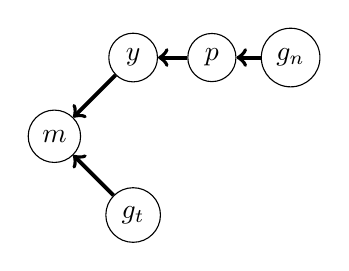
\begin{tikzpicture}[main/.style = {draw, circle}]
        \node[main] (gi) at (-1,0) {$g_n$};
        \node[main] (p) at (-2,0) {$p$};
        \node[main] (y) at (-3,0) {$y$};
        \node[main] (m) at (-4, -1) {$m$};
        \node[main] (gt) at (-3, -2) {$g_t$};
        \draw [->, line width=0.5mm] (gi) -- (p);
        \draw [->, line width=0.5mm] (p) -- (y);
        \draw [->, line width=0.5mm] (y) -- (m);
        \draw [->, line width=0.5mm] (gt) -- (m);
    \end{tikzpicture}
\end{figure}
\end{document}